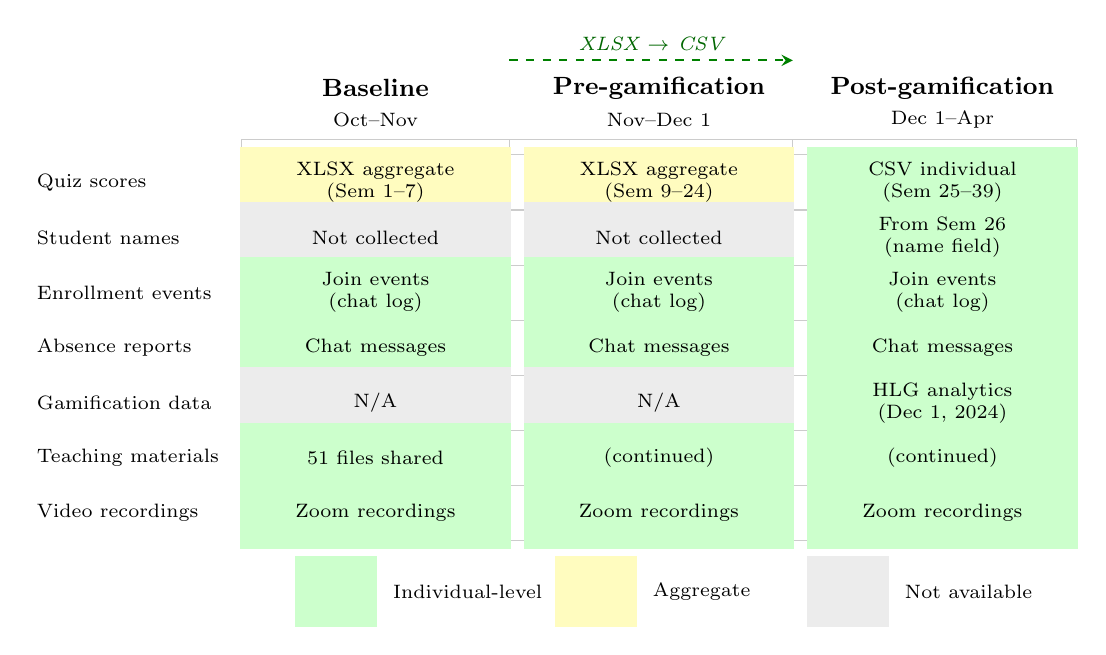
\begin{tikzpicture}[
  font=\small,
  cell/.style={minimum width=3.4cm, minimum height=0.9cm, align=center, font=\scriptsize, text width=3.2cm},
  indiv/.style={cell, fill=green!20},
  aggr/.style={cell, fill=yellow!25},
  nodata/.style={cell, fill=gray!15},
  header/.style={minimum width=3.4cm, minimum height=0.5cm, align=center, font=\small\bfseries, fill=white},
  subheader/.style={minimum width=3.4cm, minimum height=0.4cm, align=center, font=\scriptsize, fill=white},
  rowlabel/.style={minimum width=2.8cm, minimum height=0.7cm, align=left, font=\scriptsize, text width=2.6cm},
  phasearr/.style={->, >=stealth, thick, green!50!black, dashed}
]

% Column positions: row labels at x=1.0, columns at x=4.0, 7.6, 11.2
\def\cola{4.0}
\def\colb{7.6}
\def\colc{11.2}
\def\rowx{1.0}

% Column headers (two rows: title + date range)
\node[header] at (\cola, 0.2) {Baseline};
\node[subheader] at (\cola, -0.2) {Oct--Nov};
\node[header] at (\colb, 0.2) {Pre-gamification};
\node[subheader] at (\colb, -0.2) {Nov--Dec 1};
\node[header] at (\colc, 0.2) {Post-gamification};
\node[subheader] at (\colc, -0.2) {Dec 1--Apr};

% Row labels and horizontal lines
\foreach \y/\rowlbl in {
  -1.0/Quiz scores,
  -1.7/Student names,
  -2.4/Enrollment events,
  -3.1/Absence reports,
  -3.8/Gamification data,
  -4.5/Teaching materials,
  -5.2/Video recordings%
}{
  \node[rowlabel] at (\rowx, \y) {\rowlbl};
  \draw[gray!40] (2.3, \y+0.35) -- (12.9, \y+0.35);
}
\draw[gray!40] (2.3, -0.45) -- (12.9, -0.45);
\draw[gray!40] (2.3, -5.55) -- (12.9, -5.55);

% Vertical dividers
\foreach \x in {2.3, 5.7, 9.3, 12.9}{
  \draw[gray!40] (\x, -0.45) -- (\x, -5.55);
}

% Quiz scores row
\node[aggr] at (\cola, -1.0) {XLSX aggregate\\(Sem 1--7)};
\node[aggr] at (\colb, -1.0) {XLSX aggregate\\(Sem 9--24)};
\node[indiv] at (\colc, -1.0) {CSV individual\\(Sem 25--39)};

% Student names row
\node[nodata] at (\cola, -1.7) {Not collected};
\node[nodata] at (\colb, -1.7) {Not collected};
\node[indiv] at (\colc, -1.7) {From Sem 26\\(name field)};

% Enrollment row
\node[indiv] at (\cola, -2.4) {Join events\\(chat log)};
\node[indiv] at (\colb, -2.4) {Join events\\(chat log)};
\node[indiv] at (\colc, -2.4) {Join events\\(chat log)};

% Absence row
\node[indiv] at (\cola, -3.1) {Chat messages};
\node[indiv] at (\colb, -3.1) {Chat messages};
\node[indiv] at (\colc, -3.1) {Chat messages};

% Gamification row
\node[nodata] at (\cola, -3.8) {N/A};
\node[nodata] at (\colb, -3.8) {N/A};
\node[indiv] at (\colc, -3.8) {HLG analytics\\(Dec 1, 2024)};

% Materials row
\node[indiv] at (\cola, -4.5) {51 files shared};
\node[indiv] at (\colb, -4.5) {(continued)};
\node[indiv] at (\colc, -4.5) {(continued)};

% Video row
\node[indiv] at (\cola, -5.2) {Zoom recordings};
\node[indiv] at (\colb, -5.2) {Zoom recordings};
\node[indiv] at (\colc, -5.2) {Zoom recordings};

% Data format evolution arrow — placed above column headers
\draw[phasearr] (5.7, 0.55) -- node[above, font=\scriptsize\itshape, green!40!black] {XLSX $\to$ CSV} (9.3, 0.55);

% Legend
\node[indiv, minimum width=1.0cm, text width=0.8cm] at (3.5, -6.2) {};
\node[font=\scriptsize, anchor=west] at (4.1, -6.2) {Individual-level};
\node[aggr, minimum width=1.0cm, text width=0.8cm] at (6.8, -6.2) {};
\node[font=\scriptsize, anchor=west] at (7.4, -6.2) {Aggregate};
\node[nodata, minimum width=1.0cm, text width=0.8cm] at (10.0, -6.2) {};
\node[font=\scriptsize, anchor=west] at (10.6, -6.2) {Not available};

\end{tikzpicture}
